\chapter{Arquitectura y diseño}\label{ch:arquitectura-y-diseno}

En este capítulo se detallan los aspectos de diseño y arquitectura del proyecto. Para la realización de este proyecto
se han utilizado diferentes herramientas y tecnologías que se detallan en los siguientes apartados.

\section{Arquitectura}\label{sec:arquitectura}

De forma visual, la arquitectura de todo el proyecto se puede contemplar en la siguiente imagen:

\begin{figure}[H]
    \centering
    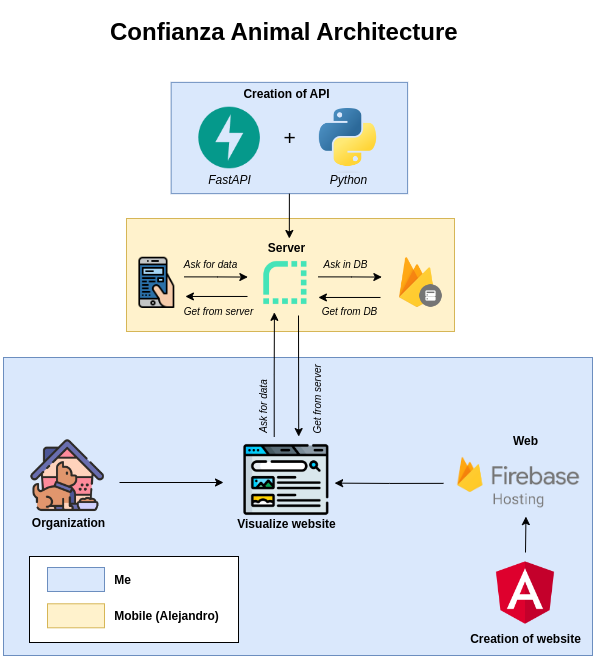
\includegraphics[width=1\textwidth]{imgs/arquitectura2.png}
    \caption{Arquitectura del proyecto}
    \label{fig:arquitectura}
\end{figure}

A primera vista, vemos que el diagrama de la arquitectura se trata de un modelo
\textbf{cliente/servidor} en el que tanto el usuario mobile (parte amarilla que referencia la arquitectura de mi compañero Alejandro)
como las organizaciones, se comunican con el servidor por medio de una API. En concreto,
la arquitectura consta de los siguientes elementos:

\newpage

\begin{itemize}
    \item \textbf{Cliente}: se trata de la página web que se comunica con la API para obtener los datos de la aplicación.
    \item \textbf{Servidor}: se trata de la API que se comunica con los servicios y la base de datos de Firebase.
    \item \textbf{Base de datos}: se trata de la base de datos en la nube de Firebase que almacena los datos de la aplicación.
    \item \textbf{Servicios}: se trata de los servicios de Firebase que se utilizan para la autenticación, el almacenamiento
    de archivos, el envío de notificaciones, etc.
\end{itemize}

El hecho de escoger esta arquitectura se debe a que es la más utilizada en la actualidad para el desarrollo de aplicaciones
web y móviles y ofrece una mayor serie de ventajas con respecto a otras alternativas como puede ser la arquitectura \textbf{peer-to-peer}
en la que los clientes se comunican entre sí sin necesidad de un servidor. Para realizar la comunicación entre el cliente
y el servidor se utiliza el protocolo HTTP. Por medio de este protocolo el cliente y el servidor pueden
intercambiar información por medio de peticiones y respuestas HTTP. \\

Al ser HTTP un protocolo sin estado, es decir, que no mantiene la información de las peticiones anteriores, permite
manejar las peticiones de forma concurrente y así mejorar el rendimiento y la escalabilidad de la aplicación. Estos
motivos hacen que su uso se haya extendido a la mayoría de las aplicaciones web y móviles. \\

Además, este tipo de arquitectura permite separar la lógica de negocio de la aplicación del cliente y alojarla en el
servidor. Esto permite que el cliente no tenga acceso a la información sensible de la aplicación y que la lógica de
negocio pueda ser reutilizada en otros clientes. También permite que el cliente pueda autenticarse para acceder a la
información del servidor y que no tenga que realizar ninguna operación de procesamiento de datos dando lugar a una
aplicación más rápida y con mejor rendimiento.

\newpage

\section{Diseño}\label{sec:diseno}

Para llevar a cabo el diseño de la aplicación se van a utilizar una serie de herramientas y tecnologías de las cuales
se ha justificado su elección en el apartado~\ref{sec:eleccion-de-herramientas-y-tecnologias}. Vamos a ver en detalle
cómo se ha planteado el diseño para la página web, la API y la base de datos:

\begin{enumerate}
    \item \textbf{Diseño de la página web}:
    \begin{itemize}
        \item En base a los requisitos del sistema, se definen los componentes y servicios que se van a utilizar en la
        aplicación.
        \item Para establecer las rutas de la aplicación se utiliza el enrutador de Angular.
        \item Para la comunicación con la API se utilizan los servicios creados y un servicio propio de Angular llamado
        \textbf{HttpClient} que permite realizar peticiones HTTP al servidor.
    \end{itemize}
    \item \textbf{Diseño de la API}:
    \begin{itemize}
        \item En base a los requisitos del sistema, se definen los endpoints que se van a utilizar en la API.
        \item Se definen los modelos de datos que se van a utilizar en la API.
        \item Se implementan los \textit{endpoints} que van a ser utilizados por la aplicación y que van
        a interactuar con la base de datos.
    \end{itemize}
    \item \textbf{Diseño de la base de datos}:
    \begin{itemize}
        \item En base a los requisitos del sistema, se definen las colecciones y estructuras de datos que se van a utilizar
        en la base de datos.
        \item Se definen las reglas de seguridad de la base de datos para que los datos estén protegidos e impedir
        accesos no autorizados.
    \end{itemize}
\end{enumerate}

Todos los detalles de implementación y despliegues que han permitido llevar a cabo la arquitectura y diseño de la aplicación se
detallan en el capítulo:~\ref{ch:implementacion-y-despliegues}.

\newpage

\section{Patrones de diseño}\label{subsec:patrones-de-diseno}

Una vez definida la arquitectura y el diseño de la aplicación, se han implementado una serie de patrones de diseño que
han ayudado a solucionar los problemas. Un patrón de diseño es una solución general y reutilizable a un problema que
ocurre con frecuencia dentro de un contexto dado en el diseño de software. Son una serie de buenas prácticas que se
pueden aplicar a cualquier proyecto de software y que permiten resolver problemas de forma más eficiente. \\

En este proyecto se han utilizado los siguientes patrones de diseño:

\begin{itemize}
    \item \textbf{Inyección de dependencias}: Se trata de un patrón de diseño que consiste en insertar las dependencias
    de un objeto en el momento de su creación. Esto permite que el objeto sea independiente de las dependencias que
    necesita para funcionar y que pueda ser reutilizado en cualquiera otra parte del código sin necesidad de crear
    una nueva instancia. Este patrón se ha utilizado para inyectar los servicios que se utilizan
    en los componentes de Angular.

    \item \textbf{Observable}: Es un patrón de diseño que permite la comunicación entre objetos de forma reactiva.
    Esto significa que cuando un objeto emite un evento, los objetos que están suscritos a ese evento son notificados
    y pueden realizar una acción. Este patrón se ha utilizado para comunicar los componentes de la web con
    los servicios y viceversa.

    \newpage

    \item \textbf{Redux}: Por medio de la librería \textbf{NgRx} se ha implementado el patrón de diseño \textbf{Redux} en la
    página web. Este patrón de diseño se basa en el concepto de \textbf{almacén centralizado} en el que se almacenan
    los datos de la aplicación. Los componentes de Angular se suscriben a los datos del almacén y cuando estos cambian
    se actualizan automáticamente. Este patrón de diseño permite que la aplicación sea escalable y que los datos
    se puedan compartir entre diferentes componentes de forma sencilla y muy rápida:
        \begin{figure}[H]
            \centering
            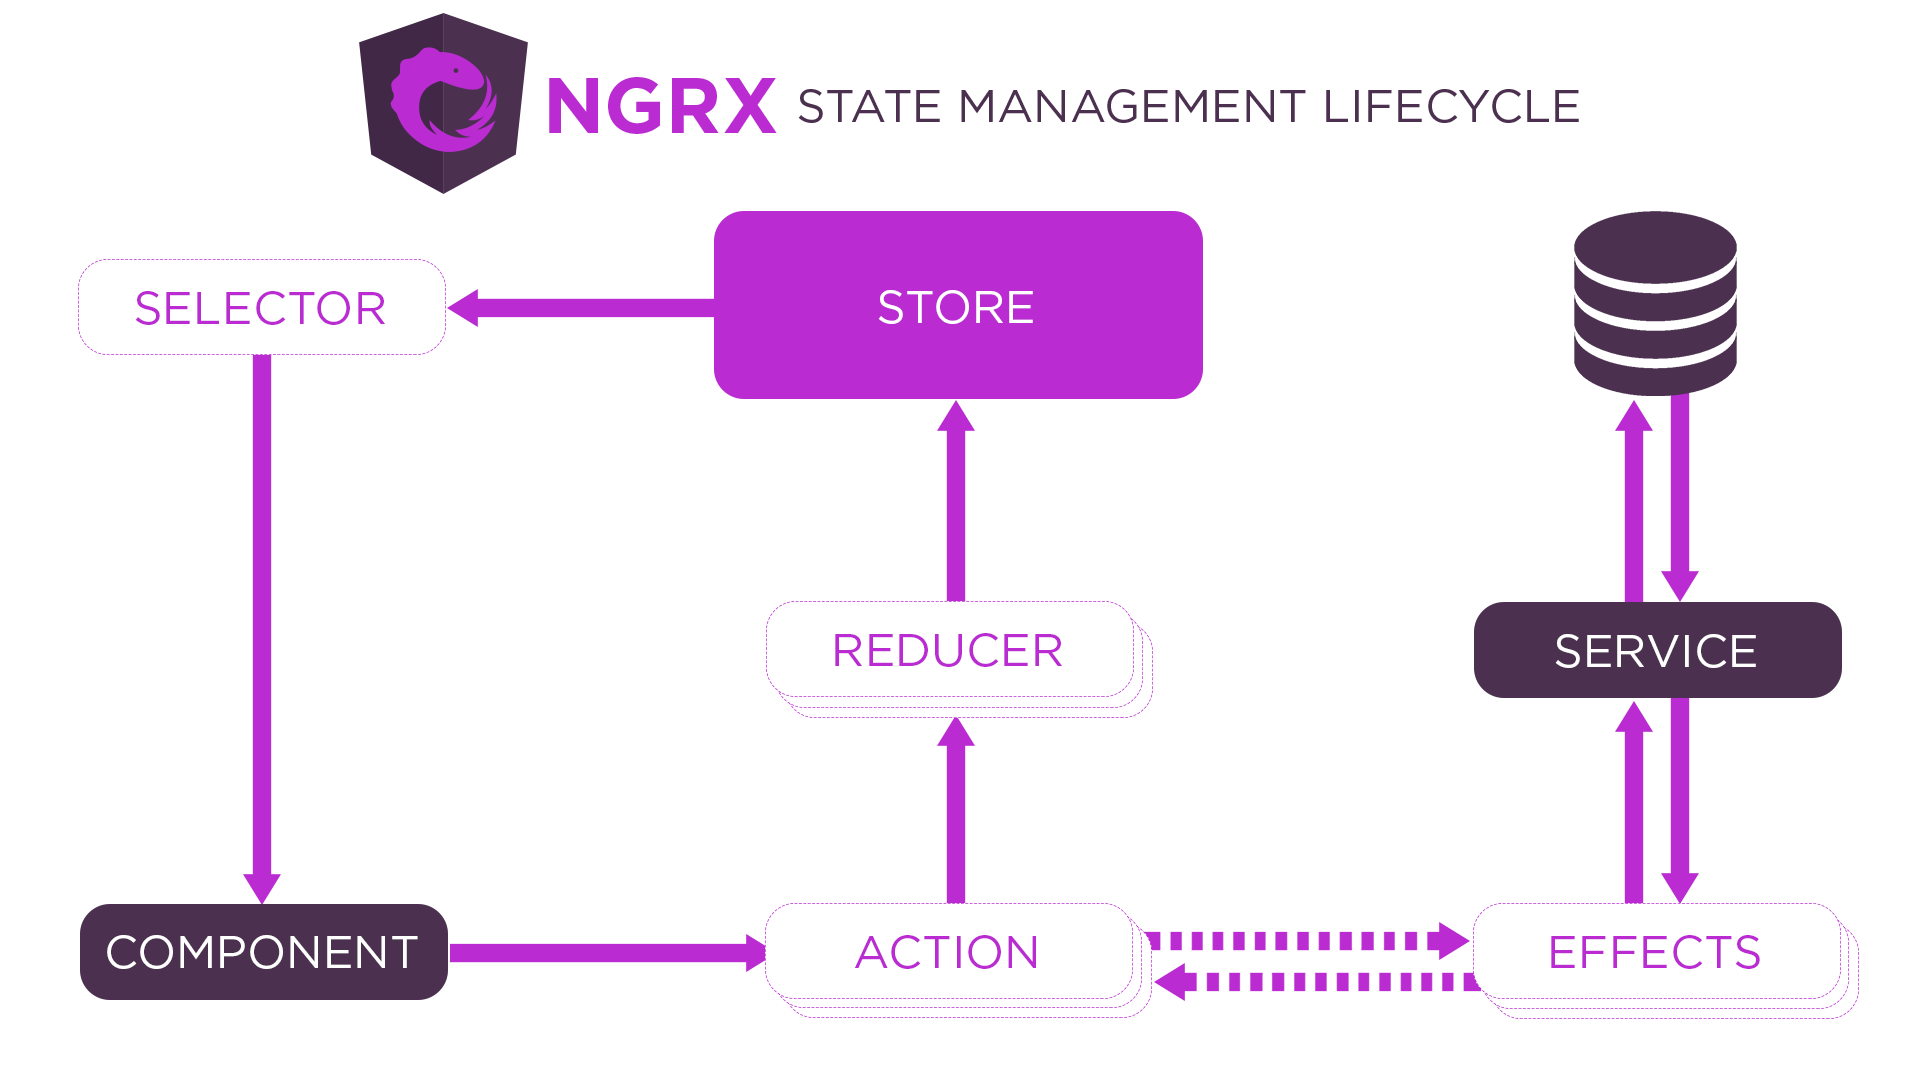
\includegraphics[width=0.9\textwidth]{imgs/ngrx.png}
            \caption{Patrón Redux con NgRx. Fuente~\cite{ngrx}}
            \label{fig:redux}
        \end{figure}
    \item \textbf{Factory method}: Este patrón de diseño se utiliza para crear objetos de una misma clase de forma
    sencilla y rápida y encapsular la lógica de creación de los objetos.

    \newpage

    \item \textbf{MVC}: Este patrón de diseño divide la aplicación en tres capas: modelo, vista y
    controlador (MVC). El modelo representa la lógica de negocio de la aplicación, la vista es la interfaz de usuario
    y el controlador es el encargado de gestionar las peticiones del usuario y comunicar los datos del modelo con la vista.
    La mejor forma de conocer el funcionamiento de este patrón de diseño es a través de una imagen explicativa:
        \begin{figure}[H]
            \centering
            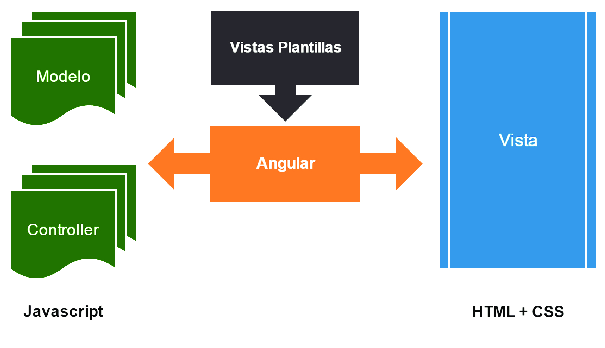
\includegraphics[width=0.9\textwidth]{imgs/mvc.png}
            \caption{Patrón MVC. Fuente~\cite{mvc}}
            \label{fig:mvc}
        \end{figure}
    \item \textbf{Composite}: Este patrón de diseño se utiliza para crear estructuras jerárquicas de objetos. En este
    proyecto se ha utilizado para crear la estructura jerárquica de los diferentes tipos de animales que se pueden
    englobar en una categoría denominada \textit{Animal}.
\end{itemize}